\begin{problem}

	\begin{wrapfigure}{r}{0.3\textwidth}
	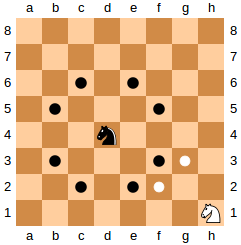
\includegraphics[width=0.28\textwidth]{skak_riddari.png}
	\end{wrapfigure}

	Við erum með venjulegt skákborð af stærð $8\times 8$. Raðir skákborðsins eru merktar með tölustöfunum $1$ til $8$ (í hækkandi röð), og dálkar skákborðsins eru merktir með bókstöfunum \texttt{a} til \texttt{h} (í hækkandi stafrófsröð). Þá getum við talað um reiti með rithætti eins og "`\texttt{e5}"', en það merkir reitinn sem er staðsettur í dálki \texttt{e} og röð $5$.

	Við erum líka með einn riddara. Riddarar geta tekið skref sem eru í laginu eins og stafurinn \texttt{L}. Þeir geta gengið áfram um tvo reiti í einhverja af fjórum aðal áttunum (ekki á ská), og tekið svo eitt skref í aðra hvora áttina sem er hornétt á áttina sem hann fór fyrst í. Athuga skal að riddarinn má ekki taka skref útaf skákborðinu. Þetta er eins og hefðbunda hreyfingin sem riddari getur tekið í hefðbundinni skák.

	Skrifið forrit sem les inn upphafsreit riddarans og endareit riddarans. Forritið á að finna stystu leið fyrir riddarann til að fara frá upphafsreitinum til endareitsins. Ef fleiri en ein leið kemur til greina er nóg að skrifa út eina þeirra. Leiðinni á að vera lýst með reitunum sem riddarinn á að fara á, í sömu röð og hann fer á þá.

\begin{example}
\exmp{%
Upphafsreitur: \underline{a1}
Endareitur: \underline{b2}
Stysta leið: a1 b3 d2 c4 b2
}%
\end{example}
\begin{example}
\exmp{%
Upphafsreitur: \underline{b5}
Endareitur: \underline{b5}
Stysta leið: b5
}%
\end{example}
\begin{example}
\exmp{%
Upphafsreitur: \underline{h8}
Endareitur: \underline{a1}
Stysta leið: h8 f7 e5 c4 a3 c2 a1
}%
\end{example}
\end{problem}